\documentclass[letterpaper,12pt]{article}
\usepackage{tabularx} % extra features for tabular environment
\usepackage{amsmath}  % improve math presentation
\usepackage{amsfonts}
\usepackage{verbatim}
\usepackage{graphicx} % takes care of graphic including machinery
\usepackage[margin=1in,letterpaper]{geometry} % decreases margins
\usepackage{cite} % takes care of citations
\usepackage[final]{hyperref} % adds hyper links inside the generated pdf file
\hypersetup{
	colorlinks=true,       % false: boxed links; true: colored links
	linkcolor=blue,        % color of internal links
	citecolor=blue,        % color of links to bibliography
	filecolor=magenta,     % color of file links
	urlcolor=blue         
}
\usepackage{blindtext}

\usepackage{units}
\usepackage{lineno}
%++++++++++++++++++++++++++++++++++++++++


\begin{document}
\linenumbers
\title{Uncertain Effects of DFT Functionals on Calculations of Organic semiconductor Charge Mobility}
\author{authors}
\date{\today}
\maketitle

\begin{abstract}
    We study the uncertainty effect from the DFT functional to the charge mobility calculations of organic semiconductors (OSC). 
    The ToF mobilities of the BCP and MADN devices are calculated from the first principle multiscale model. 
    BCP has a large energy disorder while MADN has a small energy disorder.
    Using a total of 10 different DFT functionals, we find that the electronic structure properties have similar distributions as indicated by Wasserstein distance, while the charge mobility of the could have a relatively large deviation.
    Further investigation reveals that ToF can be sensitive to the energy of a single node, leading to the ToF being sensitive to DFT functionals.
    And those nodes are effectively trap nodes.
    Further investigation reveals that the BHANDHLYP functional leads to a trap site, and the charge mobility is very sensitive to the trap sites' energy, so a small change in the site's energy results in a large deviation of ToF.  

    We further investigate the uncertainty effect of electronic structure properties on the charge mobility 
    We find that the site energy has the most significant effect on the charge mobility and a confidence level of charge mobility is obtained encoding the maximum amount of uncertainty in electronic structure parameters. 
\end{abstract}

\section{Introduction}
Charge mobility is one of the main quantities of interest for OSC.

Since the charge transport in OSC involves electrons, quantum mechanics and Schr\"odinger equation are essential for the theoretical study of charge mobility.

Charge conductance is due to electron dynamics, so quantum mechanics and Schr\"odinger equation are essential for the theoretical study of charge mobility. 

Due to the complexity of Schr\"odinger Equation, one alternative theory is the density functional theory (DFT). DFT has two challenges. Firstly, it is computationally impossible to perform electronic structure calculations for the whole OSC device. And secondly, the exchange-correlation potential in DFT has an unknown formula.

The first challenge is overcome by approximating the electron dynamics as transition processes between the localized states, with the transition rates calculated as the temperature-activated bi-molecule transition rates, known as the Marcus rate. 
The second challenge is addressed by utilizing DFT functionals to represent the exchange-correlation potential. 
Those functionals are benchmarked to achieve good consistency with many physical quantities, such as ionization potential, and density of states. 

In the framework of this multiscale model, the accuracy of the DFT functionals determine the accuracy of the calculated mobility. 

We can use the steady state mobility, 

The influence of the different functionals on ToF calculation is missing. 
In this work, we want to study how the DFT functionals affect the electronic structures and ToF charge mobility.

The goal of this work is to investigate how the DFT functionals affect the electronic structures and ToF charge mobility.
We want to answer questions: 

%%%%%%%%%%%%%%%%%%%%%%%%%%%%%%%%%%%%%%%
\section{Results}
\label{sec:result}

\subsection{Distribution Distance and ToF Differences}
A summary of the Time-of-Flight (ToF) and molecular energies using different functionals is provided in Table \ref{tab:para}, with the drift ToF detailed in Table \ref{tab:para2}. The tables indicate that while the energy standard deviations $\sigma(E)$ are similar across different functionals, the ToF values vary significantly, notably for functionals like BHANDHLYP, M06L, and BHLYP.

\begin{table}[h]
    \centering
    \begin{tabular}{c c c c c }
    \hline
        Functional & ScaleHFX & $\lambda_h$ [eV] & ToF [s] & $\sigma(E)$ \\ 
        \hline
        PBE0 & 0.25 & 0.388 & 1.23e-3 & 0.175 \\
        PBE & 0 & 0.303 & 1.04e-3 & 0.172 \\ 
        B3LYP & 0.20 & 0.375 & 4.28e-3 & 0.175 \\
        BHANDHLYP & 0.5 & 0.494 & \textbf{737.94} & 0.192 \\
        TPSS & 0 & 0.310 & 1.37e-2 & 0.168 \\
        BP86 & 0 & 0.304 & 7.46e-3 & 0.175 \\
        wB97X & 0.157 & 0.505 & 2.92e-2 & 0.191 \\
        wB97X-D3 & 0.195 & 0.496 & 4.89e-2 & 0.180 \\
        M06L & 0 & 0.312 & 3.19e-1 & 0.165 \\
        BHLYP & 0.5 & 0.493 & 2.47 & 0.192 \\
    \hline
    \end{tabular}
    \caption{Values of $\lambda_h$, ToF, stationary state velocity, and energy standard deviation of BCP molecules calculated from different functionals.}
    \label{tab:para}
\end{table}

\begin{table}[h]
    \centering
    \begin{tabular}{c c c}
    \hline
        Functional & ToF [s] & $\mu$ [m/s] \\ 
        \hline
        PBE0 & 2.39e-8 & 5.68e-5 \\
        PBE & 6.03e-9 & 2.25e-4 \\ 
        B3LYP & 1.67e-8 & 8.13e-5 \\
        BHANDHLYP & 3.36e-4 & 4.04e-9 \\
        TPSS & 1.23e-8 & 1.10e-4 \\
        BP86 & 3.77e-7 & 3.59e-6 \\
        wB97X & 1.68e-6 & 8.08e-7 \\
        wB97X-D3 & 6.92e-7 & 1.96e-6 \\
        M06L & 3.90e-3 & 3.47e-10 \\
    \hline
    \end{tabular}
    \caption{Mobility and ToF with drift electric field $6 \times 10^7$ V/m.}
    \label{tab:para2}
\end{table}

\textbf{Point 1:} To investigate the effect of different functionals $f^\text{DFT}$ on electronic structures, we compare the energies $E_i$ and couplings $J_{i,j}$ for all molecule indices $i,j$. Scatter plots in Figures \ref{fig:scatterE} and \ref{fig:scatterJ} illustrate these comparisons.

\begin{figure}[h]
    \centering
    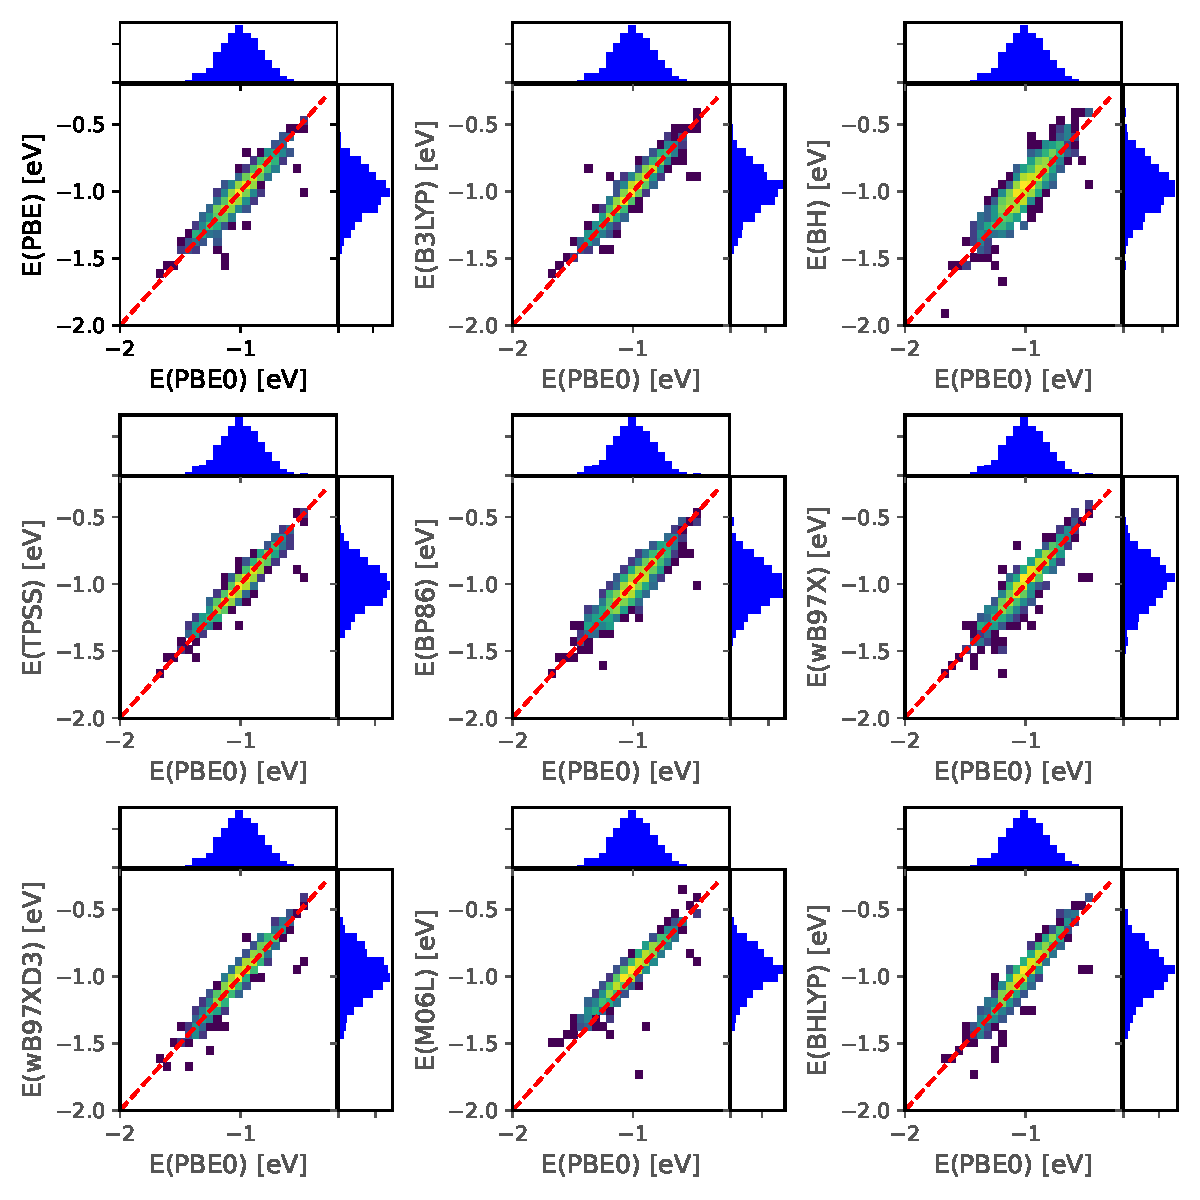
\includegraphics[width=0.95\textwidth]{figs/scatterE_all.pdf}
    \caption{Energy heat maps: $X$-axis shows energies of BCP molecules obtained using PBE0, while the $Y$-axis shows energies from a different functional $f'$.}
    \label{fig:scatterE}
\end{figure}

\begin{figure}[h]
    \centering
    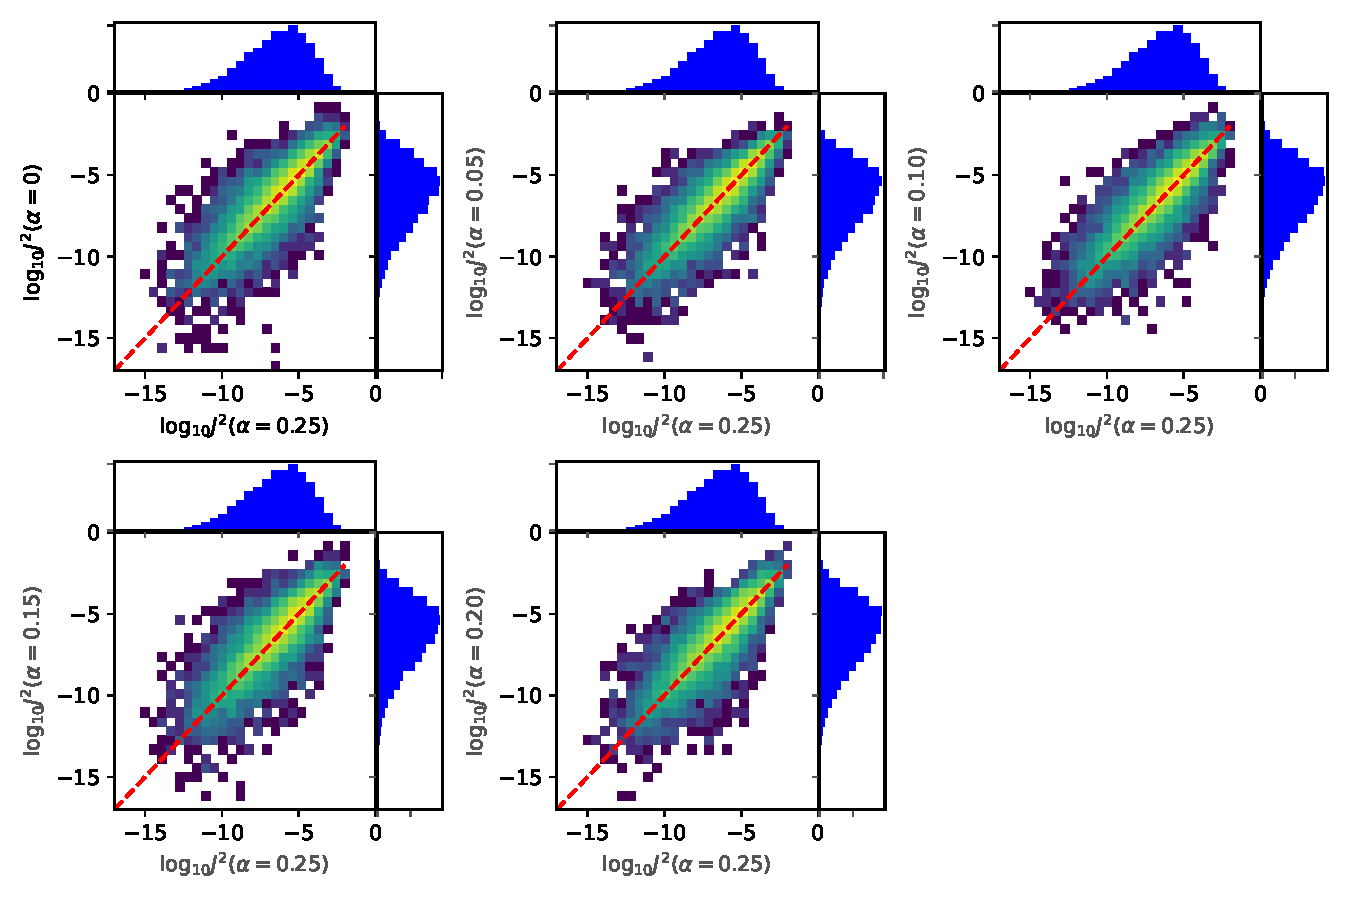
\includegraphics[width=0.95\textwidth]{figs/scatterJ_all.pdf}
    \caption{Scatter heat maps of $\log_{10}(J^2)$: $X$-axis shows $\log_{10}(J^2)$ of BCP molecules obtained using PBE0, while the $Y$-axis shows $\log_{10}(J^2)$ from a different functional $f'$.}
    \label{fig:scatterJ}
\end{figure}

\textbf{Point 2:} Both $E_i$ and $J_{i,j}$ are distributions. To quantify the impact of these distributions on $\Delta$ToF, we plot the Wasserstein distance versus $\Delta$ToF. Figure \ref{fig:distance_ToF} shows that different functionals generate similar energy sets, but $\Delta$ToF is not correlated with energy distribution distance.

\begin{figure}[h]
    \centering
    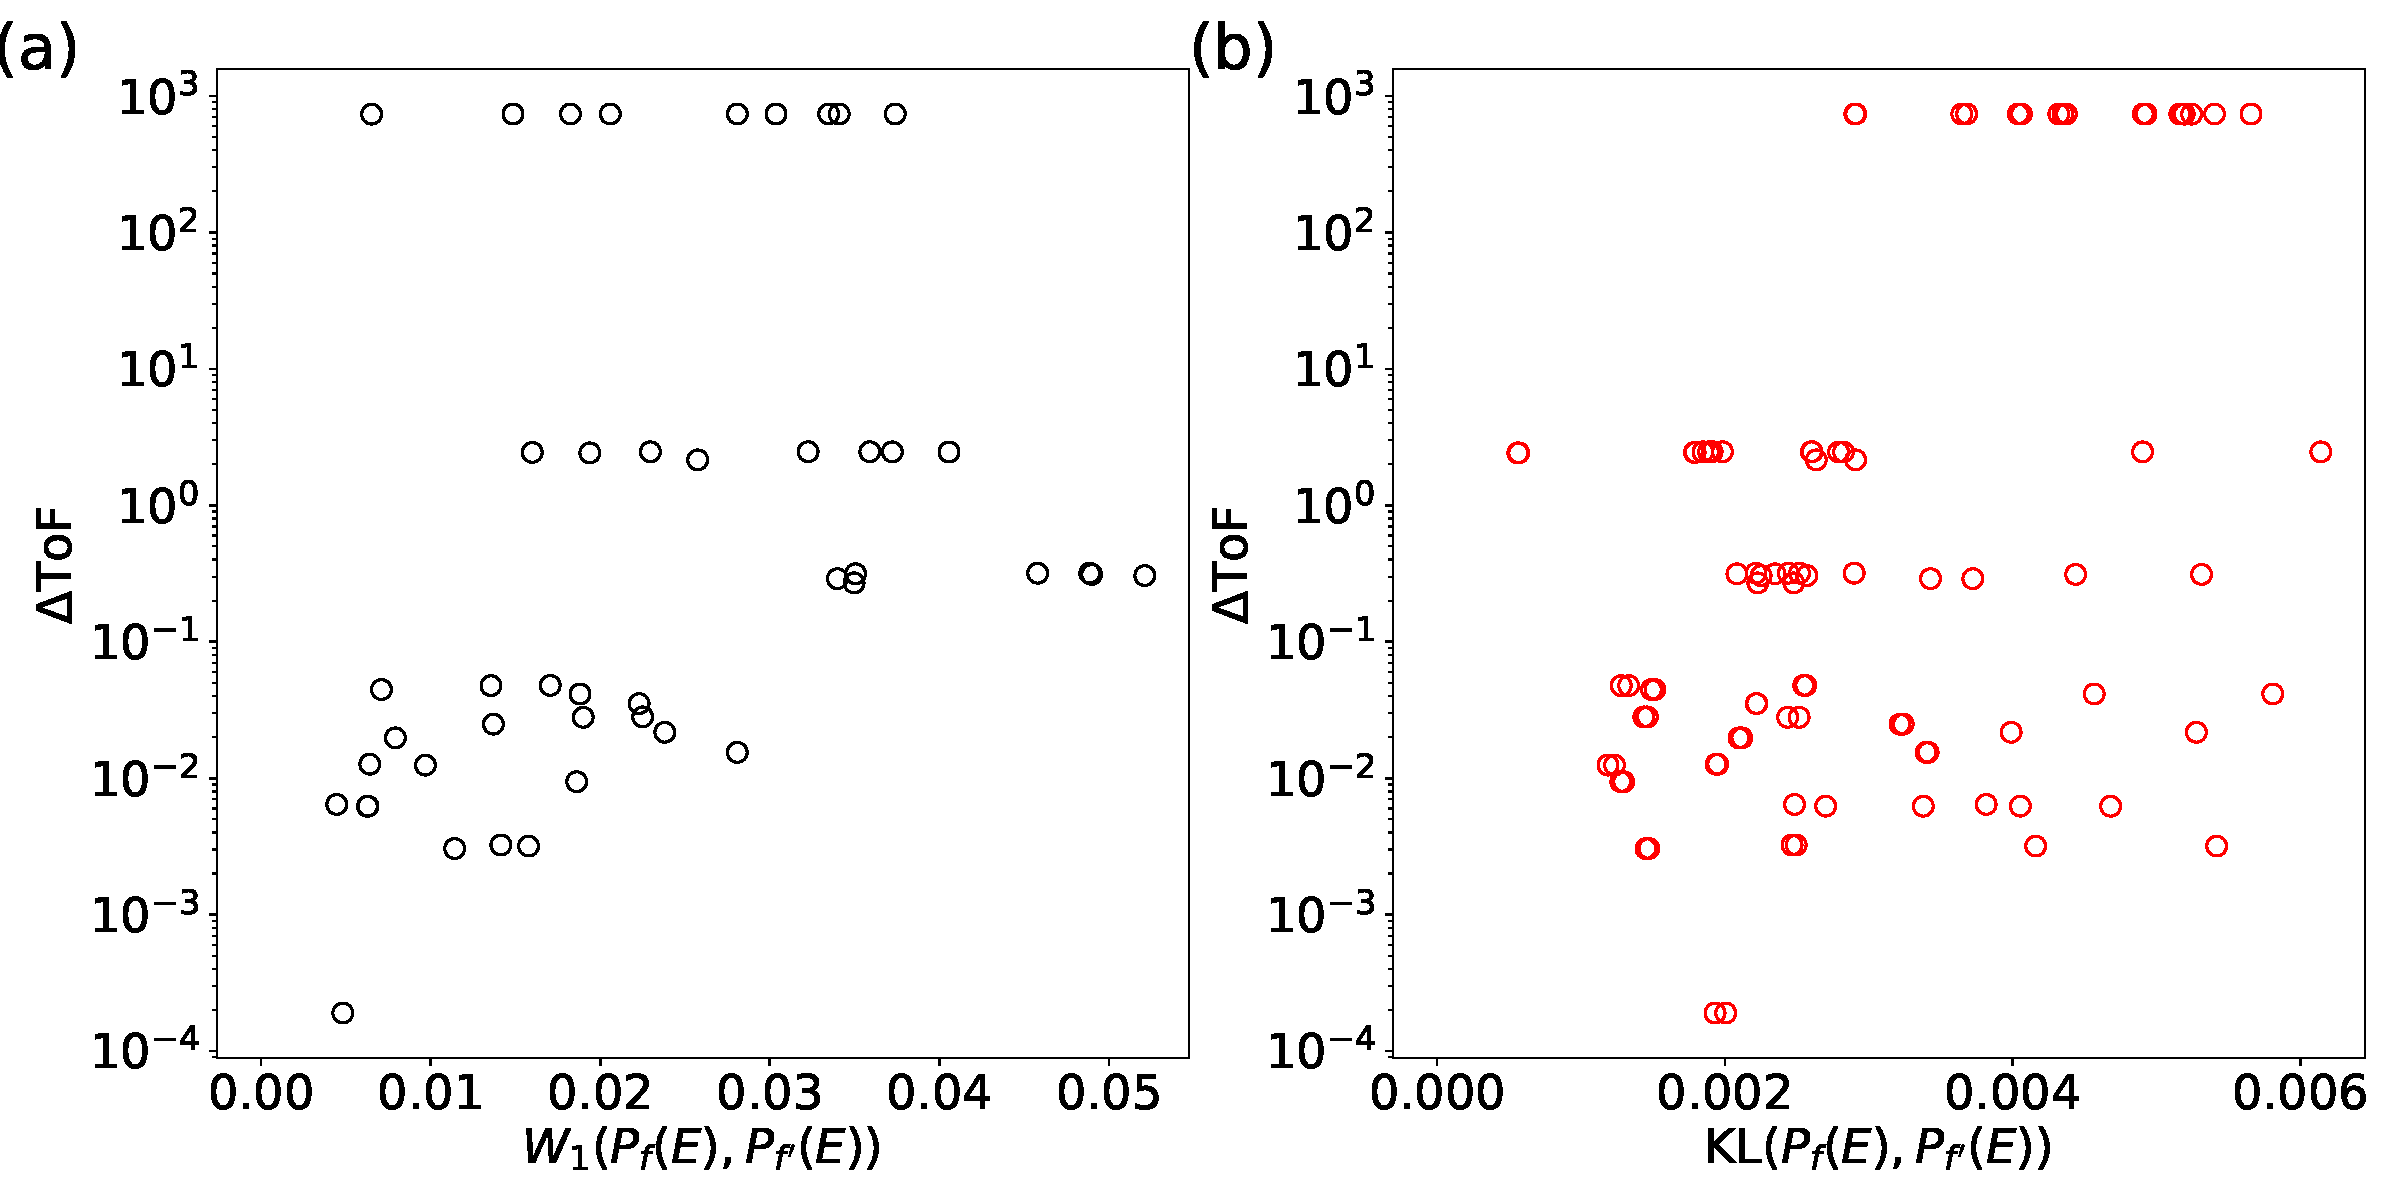
\includegraphics[width=0.9\textwidth]{figs/DeltaToF_W_KL_E.pdf}
    \caption{Left: scatter plot of $W_1(P_f,P_{f'})$ vs. $\Delta$ToF. Right: scatter plot of $KL(P_f(E),P_{f'}(E))$ vs. $\Delta$ToF.}
    \label{fig:distance_ToF}
\end{figure}

\textbf{Point 3:} We then examine other rate-related parameter distributions, calculating the Wasserstein distance and plotting against $\Delta$ToF. Figure \ref{fig:d_WD_tof} reveals that only the rate $P_f(\omega)$ has a large Wasserstein distance when varying $f^\text{DFT}$; other parameters show similar distributions.

\begin{figure}[h]
    \centering
    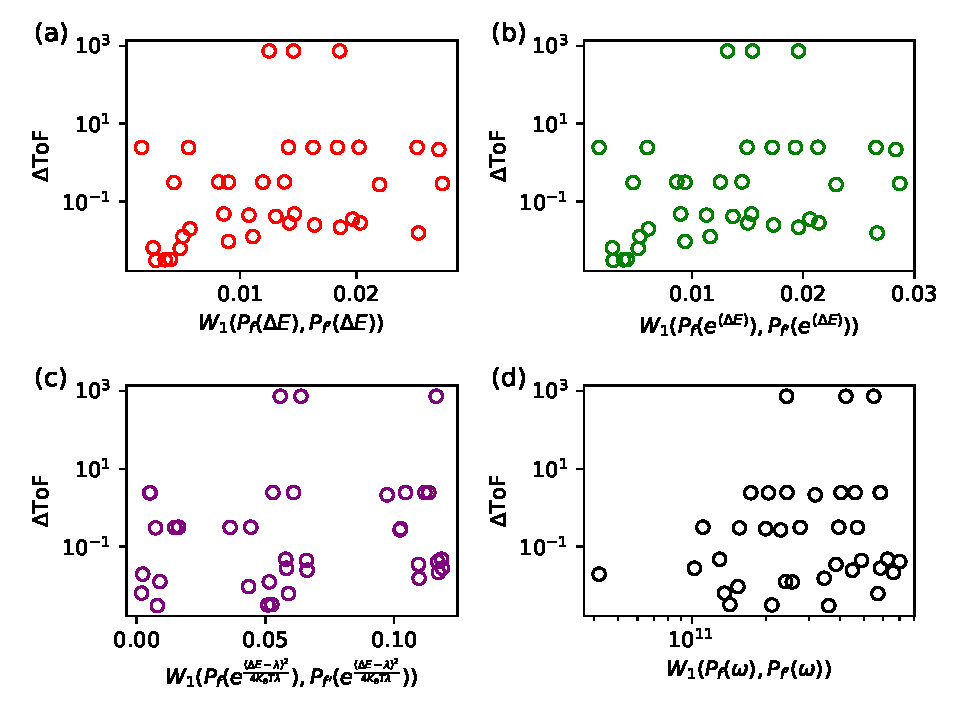
\includegraphics[width=0.7\textwidth]{figs/DeltaToF_W_all.pdf}
    \caption{Scatter plots of (a): $W_1(P_f(\Delta E),P_{f'}(\Delta E))$, (b): $W_1(P_f(\exp(\Delta E)),P_{f'}(\exp(\Delta E)))$, (c): $W_1(P_f(\exp \frac{-(\Delta E - \lambda)^2}{4 k_B T \lambda}),P_{f'}(\exp \frac{-(\Delta E - \lambda)^2}{4 k_B T \lambda}))$, and (d): $W_1 (P_f(\omega), P_{f'}(\omega) )$ vs. $\Delta$ToF.}
    \label{fig:d_WD_tof}
\end{figure}


\textbf{Point4:} Although $f^\text{DFT}$ affects $P_f(\omega)$, but we further notice that $\Delta$ToF is not correlated to its Wasserstein distance. 
So we hypothesize that the connectivity of the graph changed due to different $f^\text{DFT}$. The connectivity of the graph is quantified by the second eigenvector of the graph Laplacian, so we make the figure to investigate the correlation between the $\Delta$ToF and the graph connectivity. 
Figure .\ref{fig:d_eig_tof} shows the ratio of $f^\text{DFT}$ and the second eigenvalue ratio between the graph Laplacian. These two quantities look correlated, and we calculate the Spearman rank coefficient, which is shown in Table.\ref{tab:spearman}.

\begin{table}[h]
    \centering
    \begin{tabular}{c c c}
    \hline
        Data Set & Spearman Rank Coefficient & $p$-value \\ 
        \hline
        $\frac{\lambda_{2,L_W}(f)}{\lambda_{2,L_W}(f')}$ vs $\frac{\text{ToF}(f)}{\text{ToF}(f')}$ & -0.57 & 4.6e-5 \\
        $\frac{\lambda_{2,L_\text{rw}}(f)}{\lambda_{2,L_\text{rw}}(f')}$ vs $\frac{\text{ToF}(f)}{\text{ToF}(f')}$ & -0.38 & 9.4e-3 \\ 
    \hline
    \end{tabular}
    \caption{Spearman rank coefficients for the relationship between $\frac{\lambda_2(f)}{\lambda_2(f')}$ and $\frac{\text{ToF}(f)}{\text{ToF}(f')}$}
    \label{tab:spearman}
\end{table}

\begin{figure}[h]
    \centering
    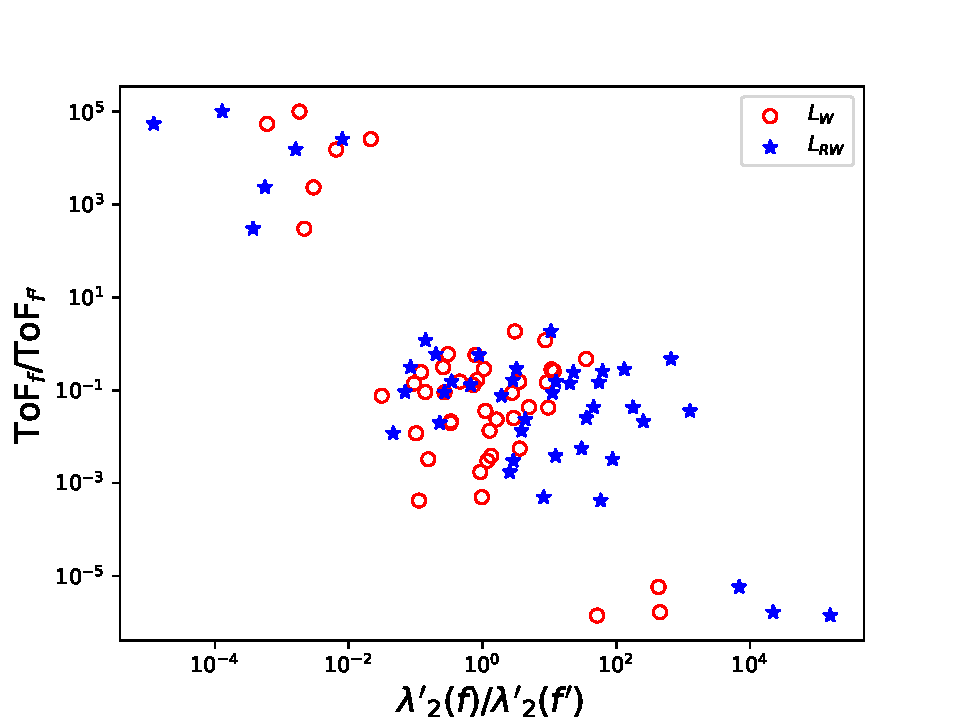
\includegraphics[width=0.6\textwidth]{figs/ratio_tof_2ndEigval.pdf}
    \caption{Scatter plot of $\frac{\lambda_{2}(f)}{\lambda_{2}(f')}$ vs. $\frac{\text{ToF}(f)}{\text{ToF}(f')}$}
    \label{fig:d_eig_tof}
\end{figure}


\textbf{Point5:} The eigenvalue comes in pair with the eigenvector, so we further investigated the corresponding second eigenvector element distributions, as shown in Fig.\ref{fig:2ndVecLW}. 
To our surprise, node 66 has very different second eigenvector entries, so we performed K-means partitioning on those second eigenvector elements.

\textbf{Point6:} After partitioning, we notice that the partition cost function is correlated to $\Delta$ToF.
This correlation shows that the $\Delta$ToF correlated to the connectivity of the graph, althouth the electronic structures and rate-related parameters are similar. 

\begin{figure}
    \centering
    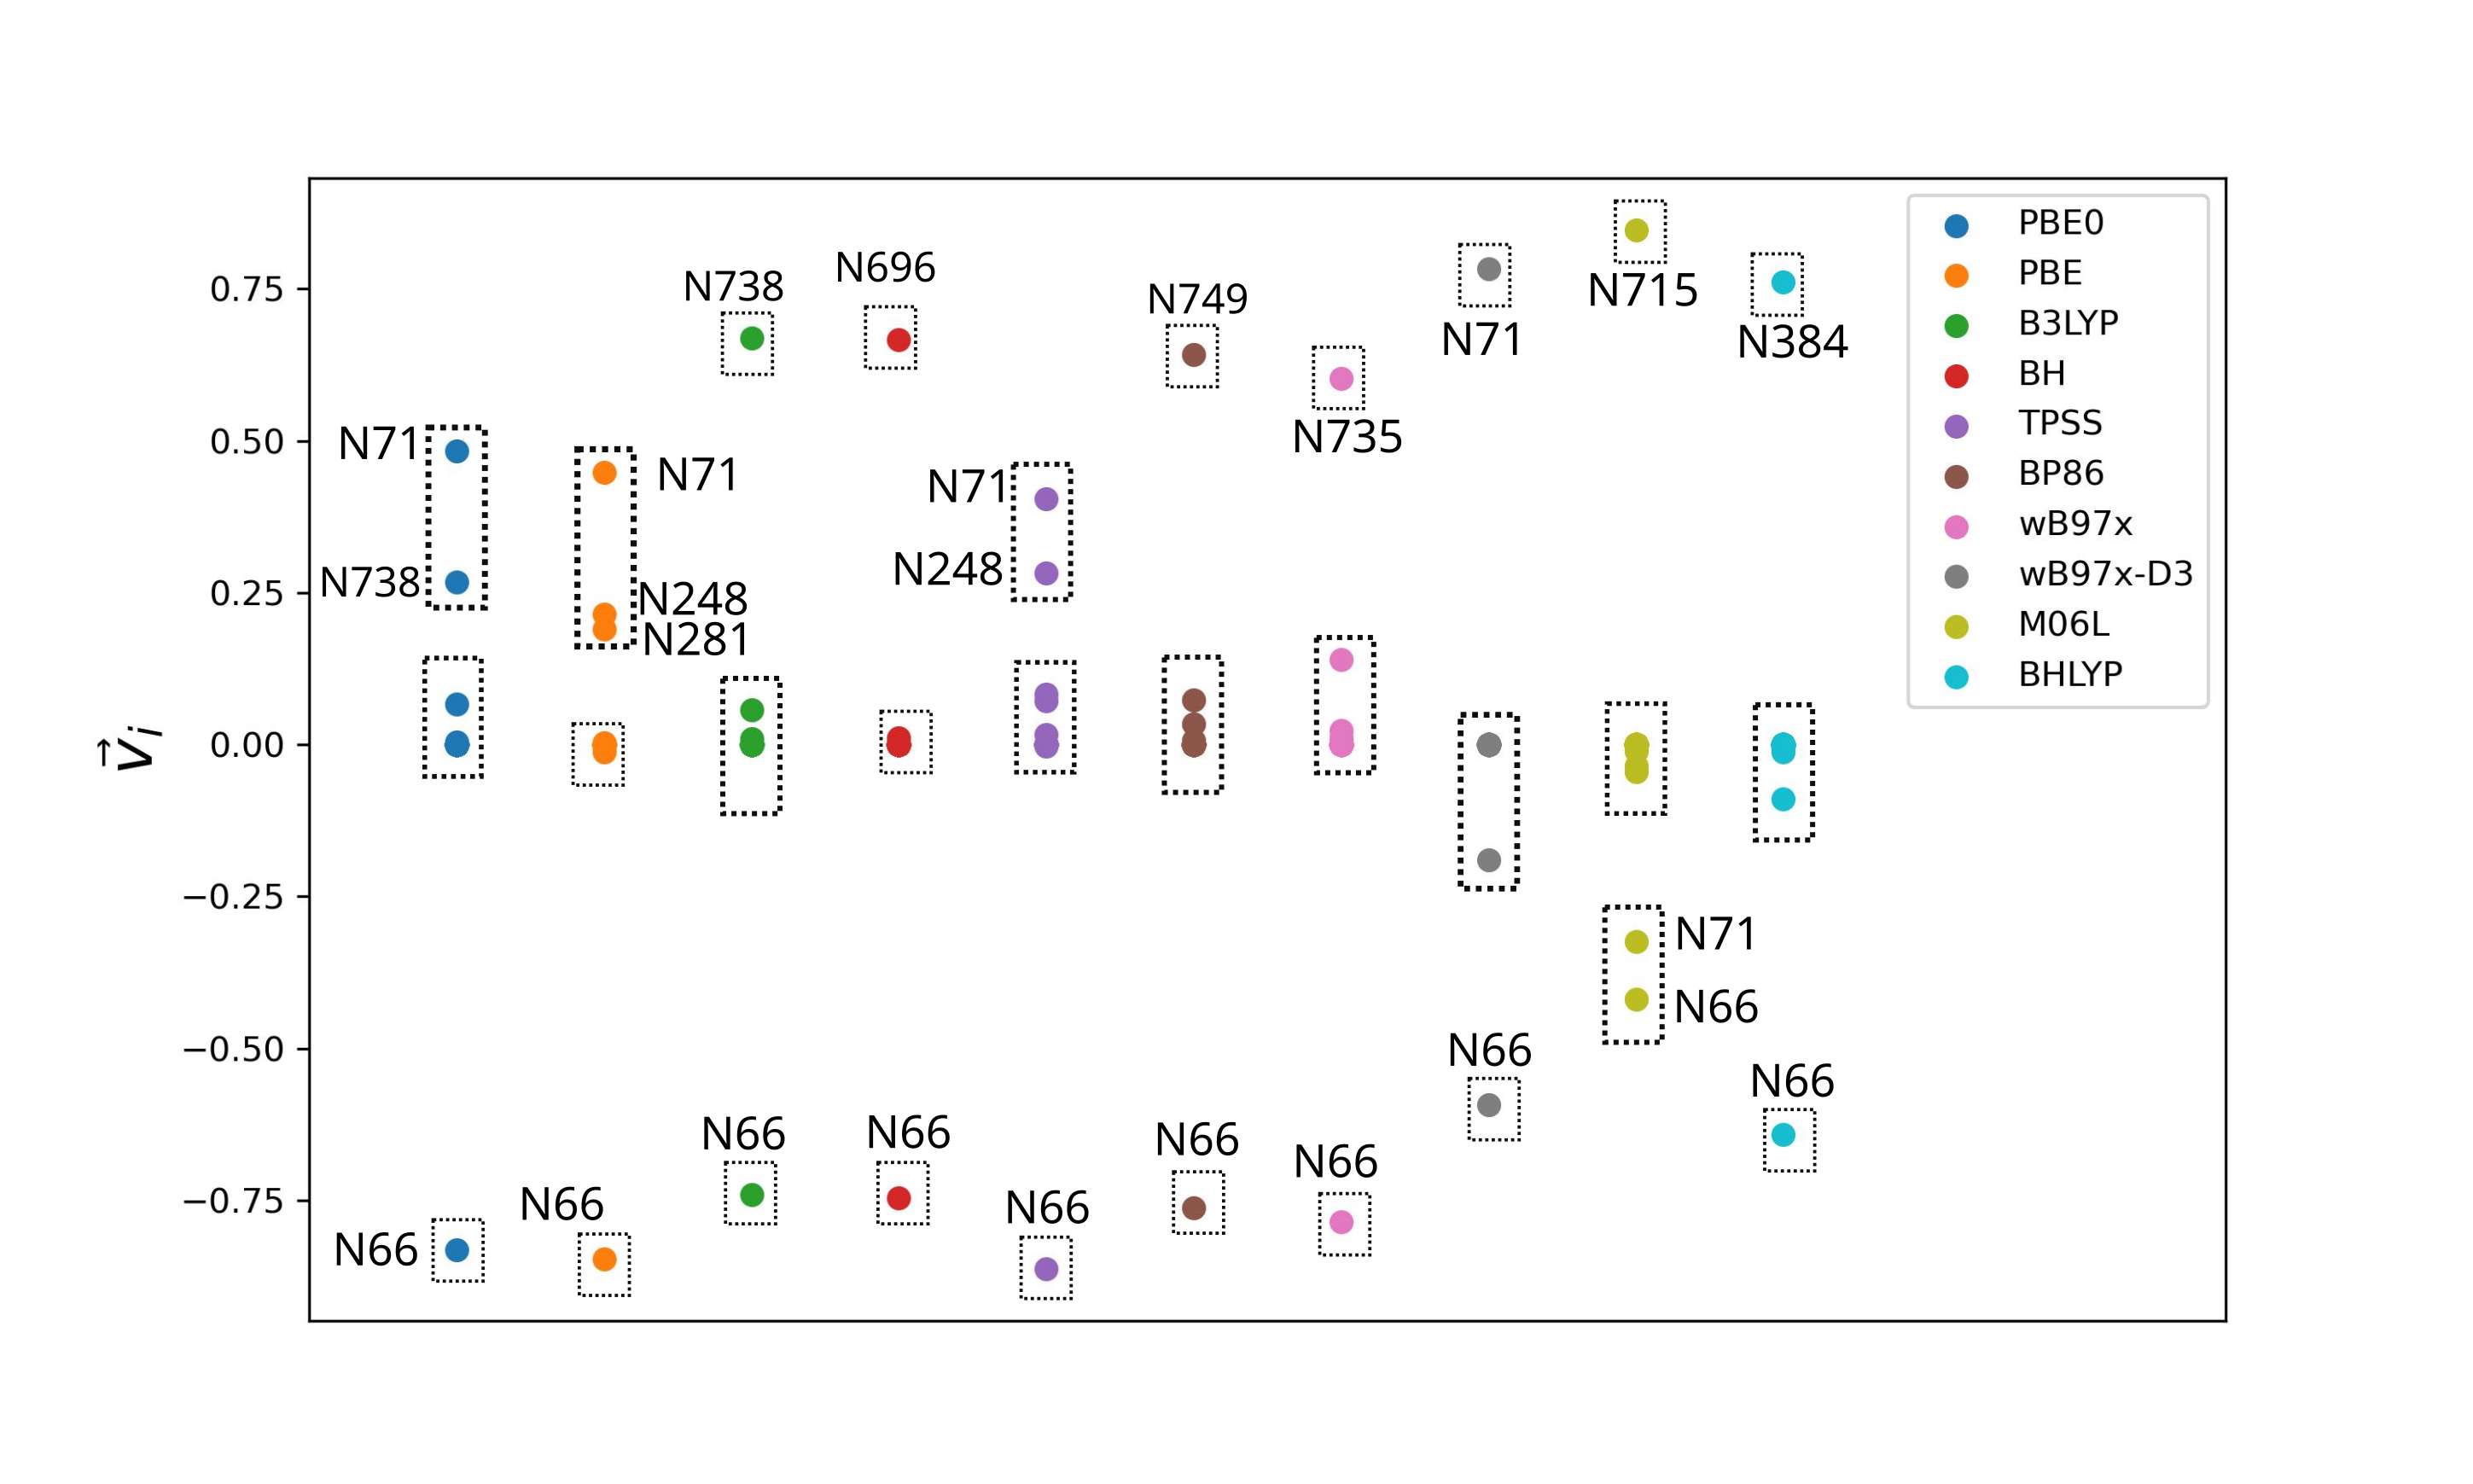
\includegraphics[width=0.8\textwidth]{figs/fig_2ndVecLw.png}
    \caption{Scatter plot of the eigen vector entries $\Vec{v}_i$ of $L_W$ for various $f$ indicated by the legend and point color. 
    The numbers are node index. The dash rectangular indicates the 3-means clusters that are detected as clusters by the Kmeans Lloyd's algorithm. }
    \label{fig:2ndVecLW}
\end{figure}

\begin{figure}
    \centering
    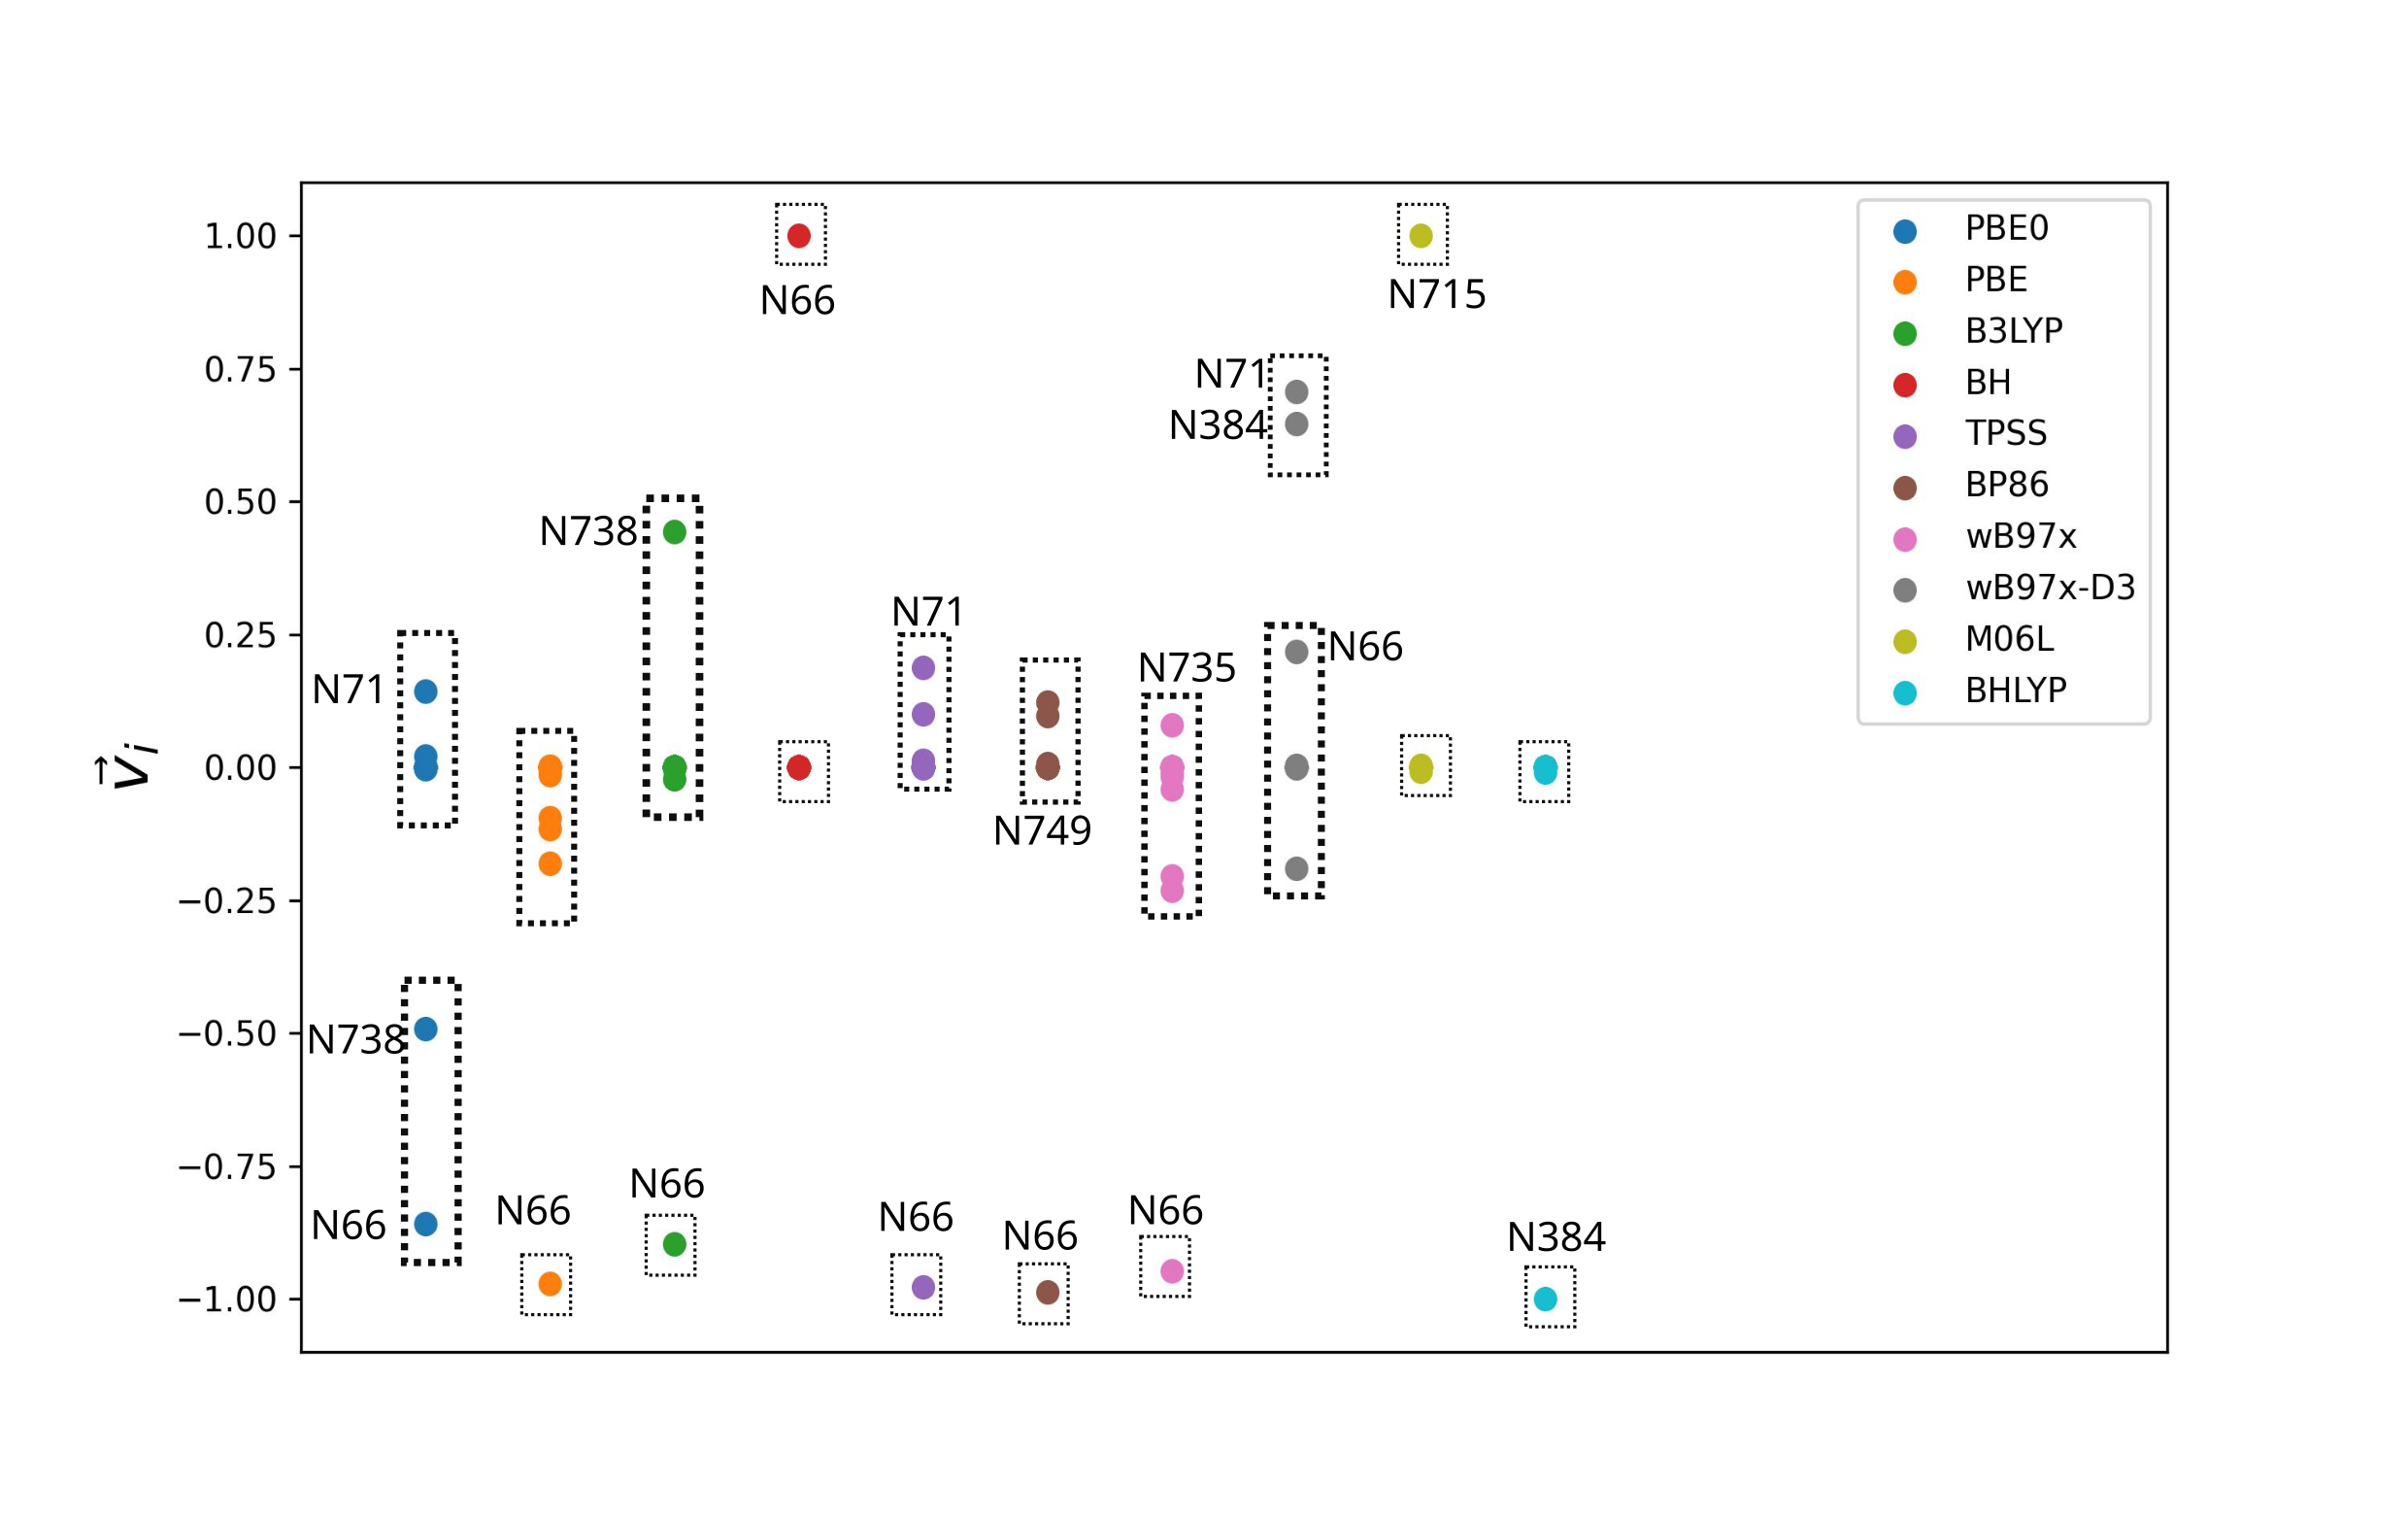
\includegraphics[width=0.8\textwidth]{figs/fig_2ndVecRW.png}
    \caption{Scatter plot of the eigen vector entries $\Vec{v}_i$ of $L_{rw}$ for various $f$ indicated by the legend and point color. 
    The numbers are node index. The dash rectangular indicates the 3-means clusters that are detected as clusters by the Kmeans Lloyd's algorithm.  }
    \label{fig:2ndVecRW}
\end{figure}


Figure \ref{fig:fig_Z_ToF} shows scatter plots of K-means clustering partition cost $Z_{2c}, Z_{3c}$ versus ToF. For the normal Laplacian $L_w$, $Z_{2c}$ is not correlated with the ToF, but $Z_{3c}$ is. For the Random-walk Laplacian, both $Z_{2c}$ and $Z_{3c}$ show a strong correlation with ToF. Thus, the clustering cost function indicates the speed of charge dynamics as measured by ToF.

\begin{figure}
    \centering
    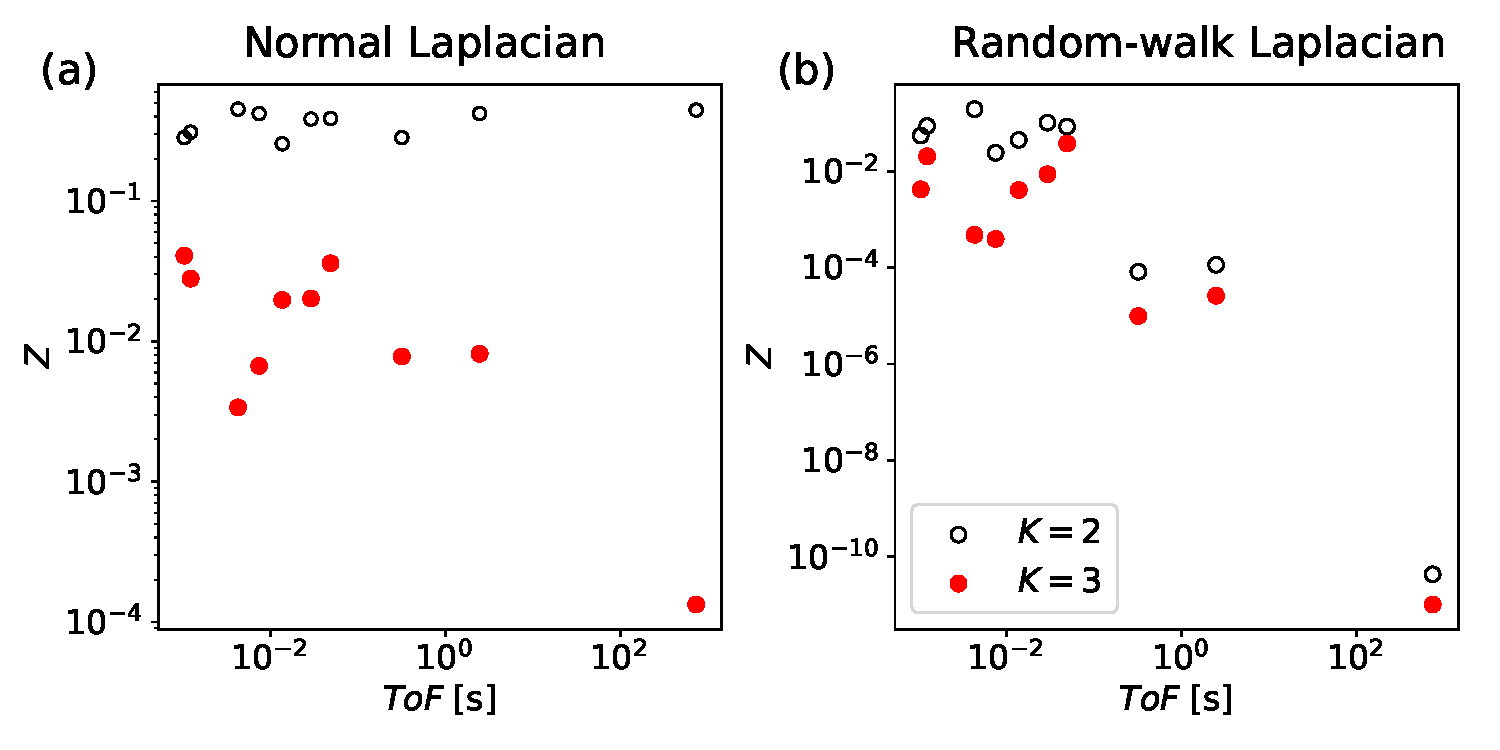
\includegraphics[width=0.9\textwidth]{figs/fig_Z_ToF.pdf}
    \caption{Scatter plot of $Z$ vs $\text{ToF}$. (a): K-means partition of the second eigenvector of $L_W$ for $K=2$ and $K=3$ (b) K-means partition of the second eigenvector of $L_{RW}$ for $K=2$ and $K=3$}
    \label{fig:fig_Z_ToF}
\end{figure} 


\textbf{Point7:} Now that the ToF has a large range, we want to know which ToF to trust.  And for application purposes, a very important message is to know what the range of ToF will give a 90\% confidence level. 

Since we do not really know the exchange-correlation potential, we assume that for each molecule, the uncertainty in its energy $E_i$ is represented by a normal distribution $E_i \in N(\bar{E_i},\sigma(E_i))$. Normal distribution is used because the normal distribution encodes the maximum amount of uncertainty over the real numbers out of all possible probability distributions with the same variance. 
So the normal distribution inserts the least amount of prior knowledge into our model. 
So we experiment: 

\textbf{Point8:} For each molecule energy $E_i$, we use maximum likelihood estimation to obtain the $N(\bar{E_i},\sigma(E_i))$. Then use sample a set of $E_i$ and calculate the ToF, with $\lambda,J_{i,j}$ fixed at the average values. 
Repeat the $E_i$ sampling and ToF calculation for 100000 times, and plot ToF distribution. This process is called the Monte Carlo sampling. 

Similarly, for $\lambda,J_{i,j}$, we perform the Monte Carlo sampling as been done for $E_i$. The resulting ToF is shown in Fig.\ref{fig:ToFs}.

\begin{figure}
    \centering
    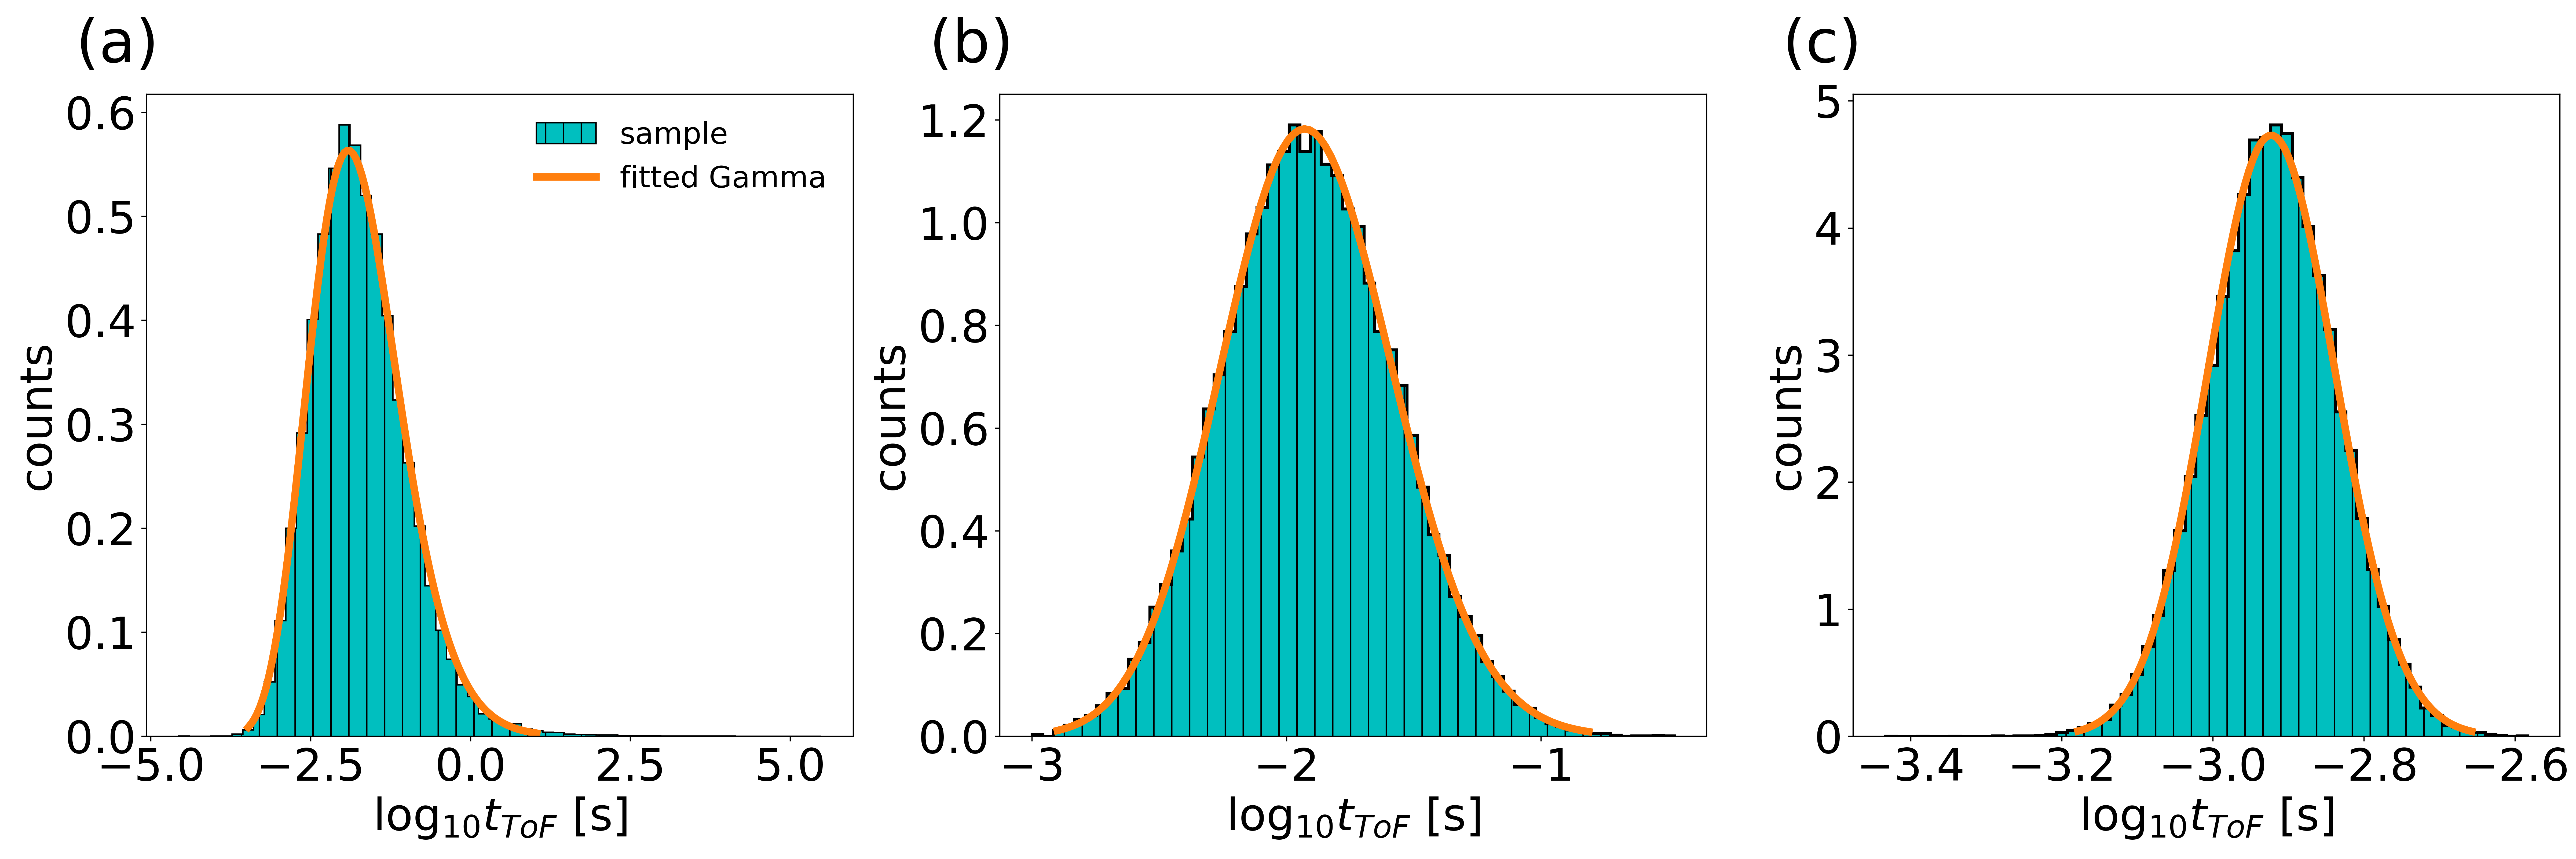
\includegraphics[width=0.9\textwidth]{figs/fig_mle.png}
    \caption{(a)The ToF distribution for 100000 samples where each $E_i$ is drawn from $N(\bar{E}_i,\sigma(E_i))$. The red curve is fitted to a gamma distribution. (b)The ToF distribution for 100000 samples where each $\lambda$ is drawn from $N(\bar{\lambda},\sigma(\lambda))$.(c)The ToF distribution for 100000 samples when each $J_{i,j}$ is drawn from $N(\bar{J_{i,j}},\sigma(J_{i,j}))$.}
    \label{fig:ToFs}
\end{figure} 

This figure shows that ToF is more sensitive to change in $E_i$ and least sensitive to $J_{i,j}$, even though from the scatter plots Fig.\ref{fig:scatterJ} the $J_{i,j}$ has a very large magnitude deviation. 

The dataset of $\log_{10}(\text{ToF})$ can be well-fitted to a Gamma distribution. 
The statistical calculation has results:
\begin{itemize}
    \item When $E_i \in N(\bar{E_i},\sigma(E_i))$, the $\log_{10}(\text{ToF})$ has mean -1.73 and a standard deviation of 0.73.
    \item When $\lambda \in N(\bar{\lambda},\sigma(\lambda))$, the $\log_{10}(\text{ToF})$ has mean -1.91 and a standard deviation of 0.34.
    \item When $J_{i,j} \in N(\bar{J_{i,j}},\sigma(J_{i,j}))$, the $\log_{10}(\text{ToF})$ has mean -2.92 and a standard deviation of 0.08.
\end{itemize}

When we use $E_i \in N(\bar{E_i},\sigma(E_i))$, $\lambda \in N(\bar{\lambda},\sigma(\lambda))$, $J_{i,j} \in N(\bar{J_{i,j}},\sigma(J_{i,j}))$ at the same to perform the Monte Carlo sampling of ToF calculation, the ToF is shown in Fig.\ref{fig:ToFs2}. the $\log_{10}(\text{ToF})$ has mean -2.72 and a standard deviation of 0.80. To obtain a 90\% confidence level, then $-3.93 < \log_{10}(\text{ToF}) < -1.30$.
\begin{figure}
    \centering
    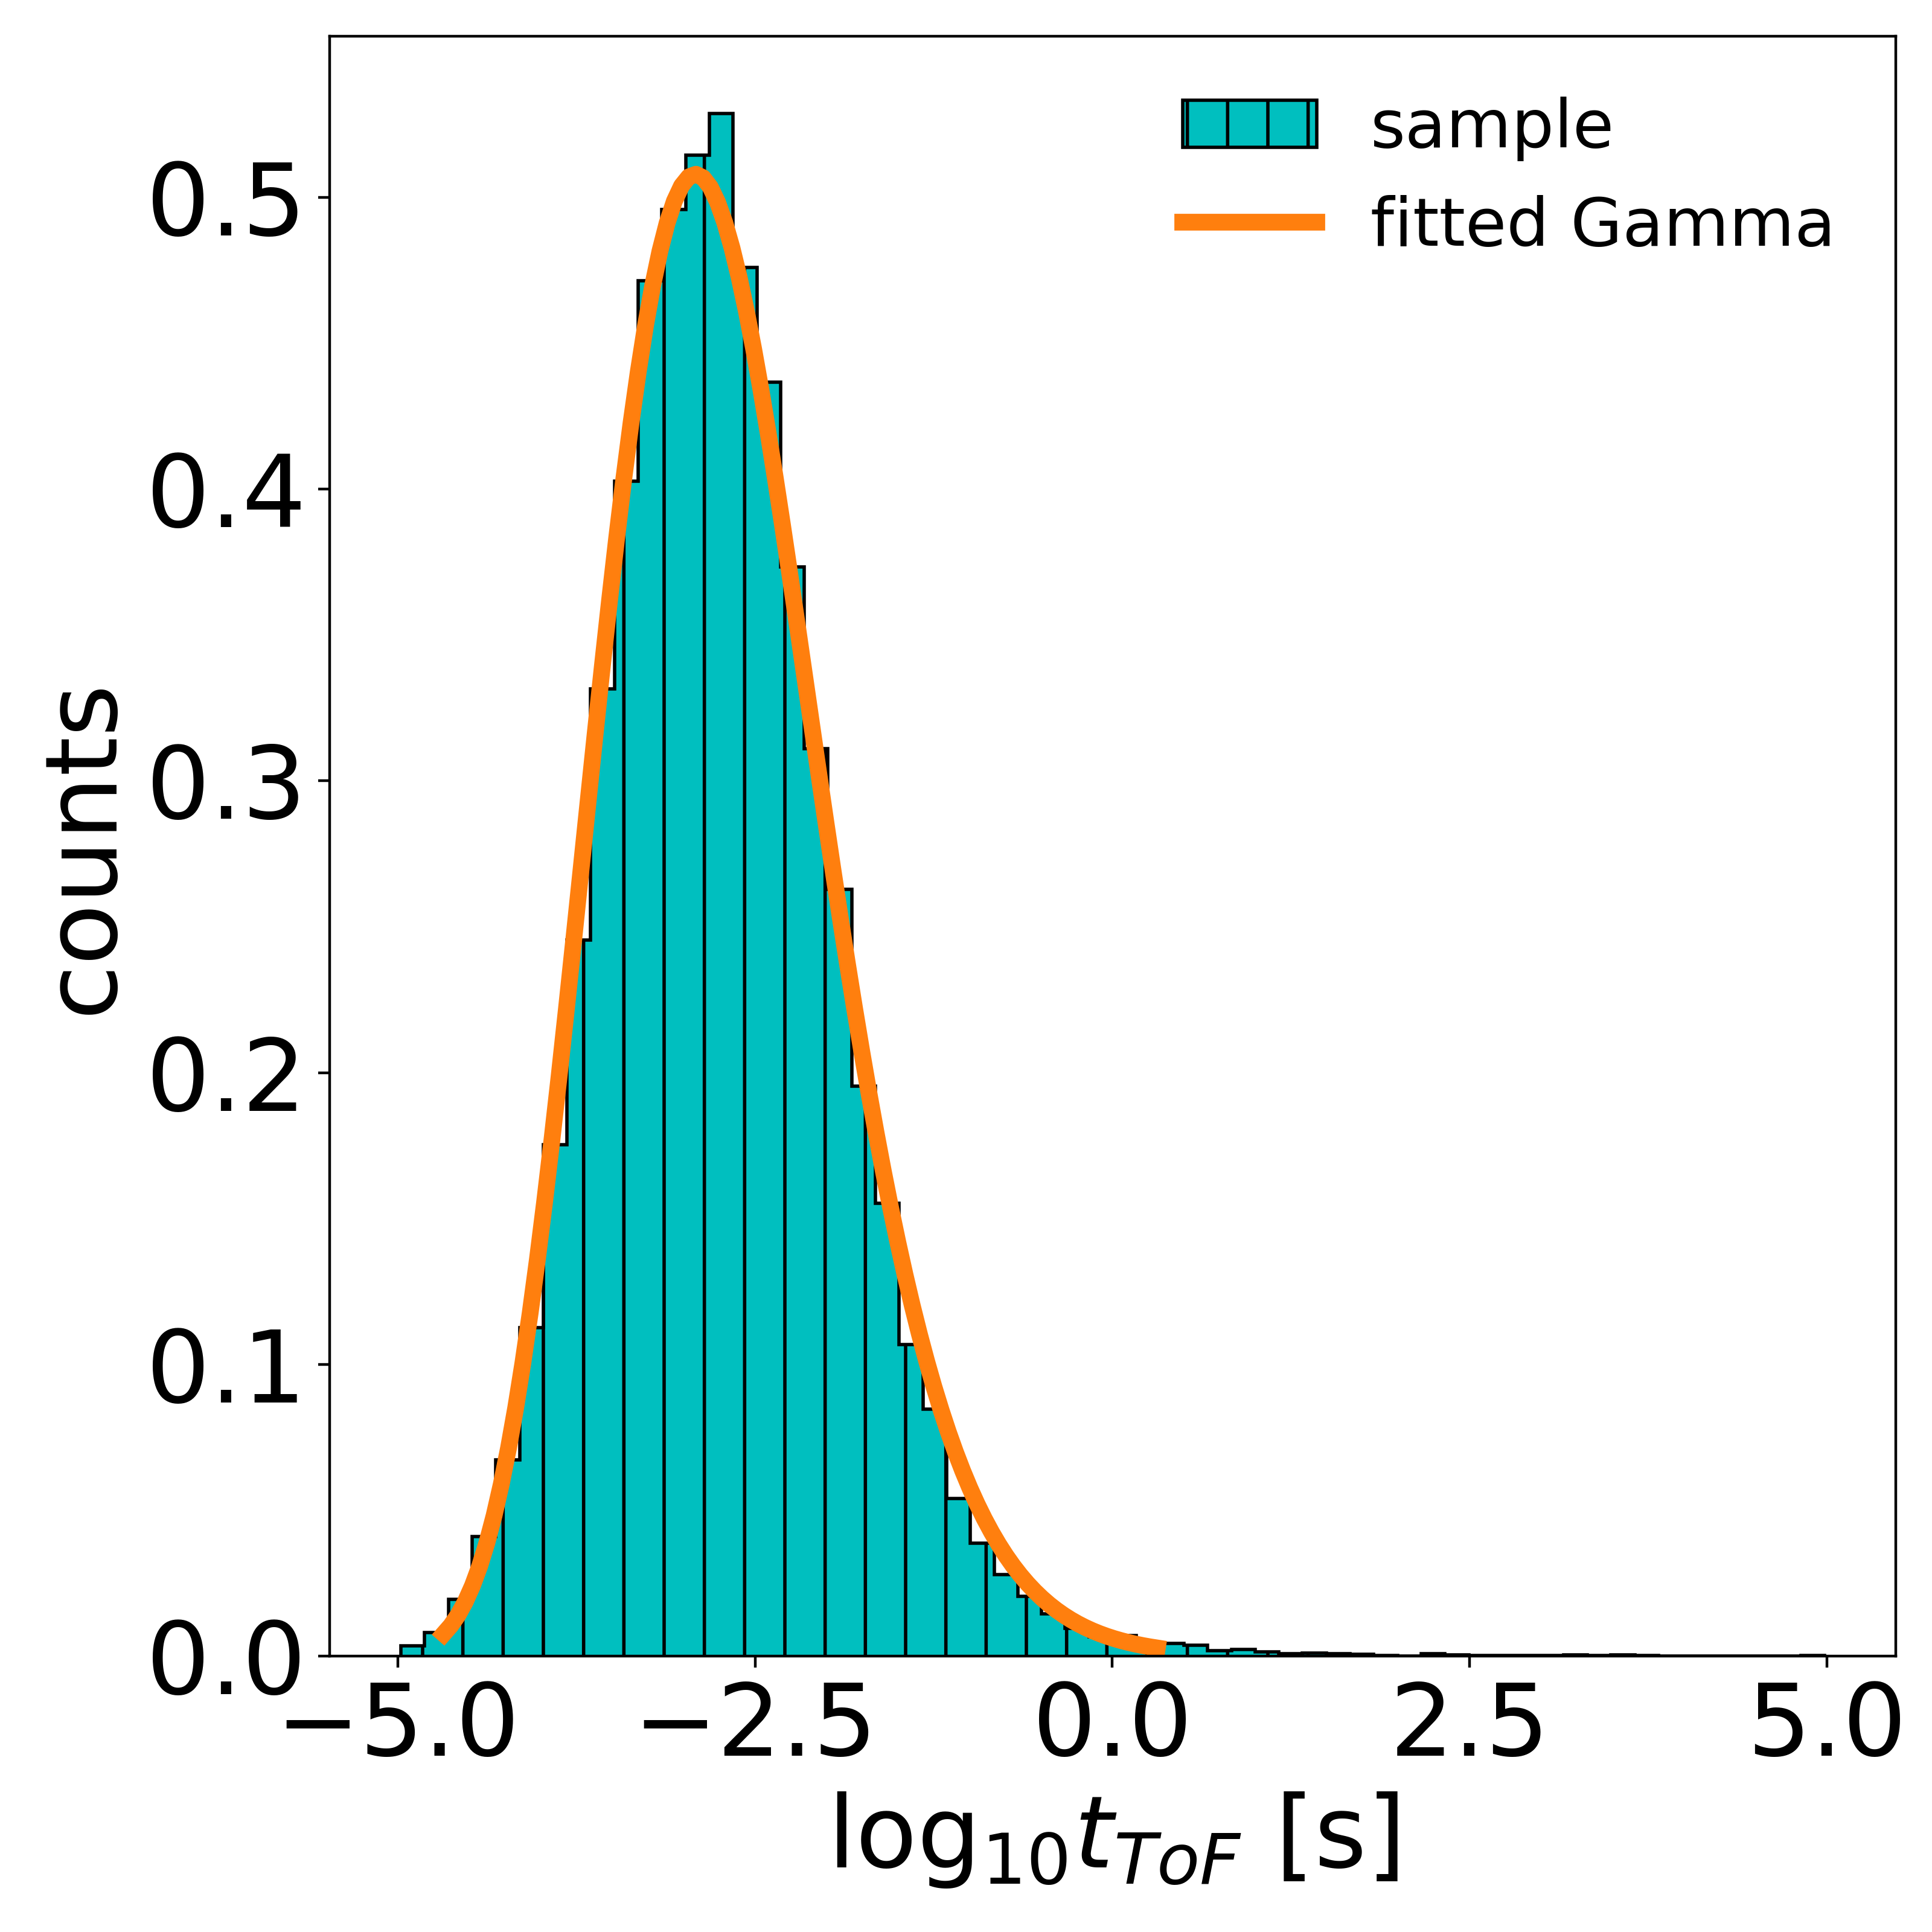
\includegraphics[width=0.6\textwidth]{figs/fig_mle2.png}
    \caption{The ToF distribution for 100000 samples where each $E_i$ is drawn from $N(\bar{E}_i,\sigma(E_i))$, $\lambda$ is drawn from $N(\bar{\lambda},\sigma(\lambda))$, and each $J_{i,j}$ is drawn from $N(\bar{J_{i,j}},\sigma(J_{i,j}))$. The red curve is fitted to a gamma distribution.}
    \label{fig:ToFs2}
\end{figure} 

%\bibliographystyle{unsrt}
%\bibliography{references}

\end{document}
